\chapter{Multi-scale modelling of dry granular flows}

\ifpdf
    \graphicspath{{Chapter4/figs/raster/}{Chapter4/figs/pdf/}{Chapter4/figs/}}
\else
    \graphicspath{{Chapter4/figs/vector/}{Chapter4/figs/}}
\fi

\section{Introduction}

The dynamics of a homogeneous granular flow involve at least three distinct 
scales: the \textit{microscopic scale}, which 
is characterised by the contact between grains, the \textit{meso-scale} that 
represents micro-structural effects such as grain rearrangement, and the 
\textit{macroscopic scale}, where geometric correlations can be observed (see 
Figure~\ref{fig:multiscale}). Conventionally, granular flows are modelled as a 
continuum because they exhibit many collective phenomena. However, on a grain 
scale, the granular materials exhibit complex solid-like and/or fluid-like 
behaviour.Recent studies, however, suggest that a continuum law may be unable 
to capture the effect of inhomogeneities at the grain scale level, such as 
orientation of force chains, which are micro-structural effects. Discrete 
element methods (DEM) are capable of simulating these micro-structural effects, 
however they are computationally expensive. In the present study, a multi-scale 
approach is adopted, using both DEM and continuum techniques, to better 
understand the rheology of granular flows and the limitations of continuum 
models.

\begin{figure}[tbhp]
\centering
\includegraphics[width=0.95\textwidth]{multiscale}
\caption{Multi-scale modelling of granular materials}
\label{fig:multiscale}
\end{figure}

\section{Granular column collapse}

The collapse of a granular column on a horizontal surface is a simple case of 
granular flow, however a proper model that describes the flow dynamics is still
lacking. Granular flow is modelled as a frictional dissipation process in 
continuum mechanics but studies showing the lack of influence of inter-particle 
friction on the energy dissipation and spreading dynamics is surprising. 
In the present study, the generalised interpolation material point method 
(GIMPM), a hybrid Eulerian -- Lagrangian approach, is implemented with 
Mohr-Coloumb failure criterion to describe the continuum behaviour of quasi-two 
dimensional collapse of granular columns. The granular column collapse is also 
simulated using DEM to understand the micro-mechanics of the flow.

~\citet{Lajeunesse2004} performed axis-symmetric and plane strain tests on 
granular column collapse. Granular materials when released suddenly on a 
horizontal surface exhibit transient flow. The mechanism of flow initiation, 
spreading dynamics and energy dissipation are studied. The experimental 
configuration used by~\citet{Lajeunesse2004} is shown in Figure~\ref{fig:exp}. 
Granular material of mass `\textit{M}' was poured into a container to form a 
rectangular heap of length `${L}_{\textit{i}}$', height `${H}_{\textit{i}}$' 
and thickness `\textit{W}'. The internal friction angle and the wall friction 
between the wall and the glass beads measured by ~\citet{Lajeunesse2004} are 
listed in Table~\ref{table:mat_prop}. The gate was then quickly removed to 
release the granular mass that spreads in the horizontal channel until it comes 
to rest. The final run-out distance `${L}_{\textit{f}}$' and the collapsed 
height `$H_{\textit{f}}$' were measured. The run-out distance and collapse 
height were found to exhibit power law relation with the initial aspect ratio 
`\textit{a}' $(=H_{\textit{i}}/L_{\textit{i}})$ of the column. 

\begin{figure}[tbhp]
\centering
\includegraphics[width=0.85\textwidth]{experiment_setup}
\caption{Schematic of experimental configuration for 2-D collapse in a 
rectangular channel,~\citep{Lajeunesse2004}}
\label{fig:exp}
\end{figure}

\begin{table}[tbhp]
\caption{Material properties of glass ballotini,~\citep{Lajeunesse2004}}
\label{table:mat_prop}
\centering
\begin{tabular}{ll}
\toprule
\textbf{Parameter} & \textbf{Value} \\ \midrule
Mean diameter & 1.15 mm \\
Repose angle & 22$\pm 0.5^{o} $\\
Avalanche angle & 27.4$\pm 0.5^{o} $\\
Wall friction angle & 24.8$\pm 0.2^{o} $\\
\bottomrule
\end{tabular}
\end{table}

\begin{figure}[tbhp]
\centering
\includegraphics[width=0.45\textwidth]{simple_shear}
\caption{Shear test periodic boundary condition}
\label{fig:shear}
\end{figure}

In this study, numerical simulations of the granular column collapse 
experiments are performed by varying the initial aspect ratio of the column. 
Discrete Element Method simulations involve modelling the granular column as 
individual particles. The granular column is prepared by randomly packing 
poly-disperse grains on a regular lattice and allowing them to undergo free 
fall due to gravity, forming a randomly packed granular column (see \mynote{Add 
Chapter reference} %TODO: Add 
%Chapter). 
The grains are allowed to reach a stable equilibrium after undergoing some 
elastic compressions due to gravity. The influence of the elastic compression 
on the energy dissipation mechanism is discussed in section \mynote{Add Section 
Reference} %TODO: ADD SECTION. 
The overlaps between particles are determined by the stiffness 
$\textit{k}_{\textit{n}}$ of the spring in the normal direction. Typically, 
average overlaps in the range 0.1 to 1.0\% are desirable and the spring 
constant is chosen to produce particle overlaps in this range. The stiffness is 
determined using the following equation:
\begin{align}
& \textit{k}_{\textit{n}}=\frac{2 \pi G}{(1-\nu)[2\ln(\frac{2r}{A})-1]} \\ 
& A = [\frac{2r(1-\nu)f_{n}}{\pi G}]^{\frac{1	}{2}}
\end{align}
where $f_{n}$ is the normal contact force; G is the shear modulus; $\nu$ is the 
Poisson's ratio and r is the radius of the grain. A simpler form of stiffness 
for a spherical grain is defined as:
\begin{align}
& \textit{k}_{\textit{n}}=4ER
\end{align}
where E is the Young's modulus of the material and R is the radius of the 
grain. The normal damping coefficient $C_{\textit{n}}$ is chosen to give a 
required coefficient of restitution $\varepsilon$ (defined as the ratio of the 
post-collisional to pre-collisional normal component of the relative velocity) 
for the materials involved:
\begin{align}
& C_{\textit{n}}=2\gamma \sqrt{m_{\textit{ij}}k_{\textit{n}}} \\ 
& \mbox{where} \quad \gamma = -\frac{\ln(\varepsilon)}{\sqrt{\pi^{2}+\ln^2 
(\varepsilon)}},\quad \mbox{and} \quad 
\textit{m}_{\textit{ij}}=\frac{\textit{m}_{\textit{i}}\textit{m}_{\textit{j}}}{\textit{m}_{\textit{i}}
 + \textit{m}_{\textit{j}}} 
\end{align}
10 Discrete Element Method simulations were carried out with columns having 
different initial aspect ratio `\textit{a}', varying from 0.2 to 10. In order 
to study the effect of crystallisation on the run-out distance, 10 more MD 
simulations were carried out on granular columns composed of grains arranged on 
a hexagonal lattice. In order to maintain a threshold amount of grains, in all 
the cases the columns contain at least 1000 grains, which is the safe lower 
limit for DEM as suggested by~\citet{Oda1999}. The micro-mechanical parameters 
used in this study are presented in Table.~\ref{table:MDdata}. Due to the 
unsteady nature of the flow, the grains get dispersed on the horizontal plane 
as discrete bodies start to separate from the main mass, hence the run-out 
distance is calculated as the position of the farthest grain which has at least 
one contact with the main mass.
\begin{table}
\caption{Micromechanical parameters used in Discrete Element Method simulations}
\label{table:MDdata}
\centering
\begin{tabular}{|l|c|}
\hline
\textbf{Parameter} & \textbf{Value} \\ \hline  \hline
Young's modulus of glass bead & $70\times10^{9}\mbox{ } N/m^{2}$ \\ \hline
Poisson's ratio & 0.22 - 0.24\\ \hline
Diameter of glass beads & 0.92 to 1.38 mm\\ \hline
Normal and shear stiffness of grains & $1.6 \times 10^{8}$ N/m \\ \hline
Normal and sear stiffness of wall & $4 \times 10^{8}$ N/m \\ \hline
Inter-particle friction coefficient, $\mu$ & 0.53 \\ \hline
Friction coefficient of wall & 0.466 \\ \hline
Coefficient of restitution, $\Gamma$ & 0.4 \\ \hline
\end{tabular}
\end{table}
A plane strain collapse of granular column is simulated as a continuum using 
MPM. The effect of number of material points on the accuracy of the simulation 
was discussed in Chapter 4.~\citet{Guilkey2003} suggests at least four 
particles per cell for problems involving large deformations. 10 MPM 
simulations of the granular column collapse were performed using Mohr-Coulomb 
constitutive law by varying the initial aspect ratio, to understand the 
difference between the particle and continuum scale description of granular 
flows. The parameters used for the continuum analyses are presented in 
Table.~\ref{table:MPMData}. The Young's modulus of the granular assembly is 
determined by performing a uni-axial compression of the granular column in 
Discrete Element Method.

\begin{table}
\caption{Parameters used in continuum simulations}
\label{table:MPMData}
\centering
\begin{tabular}{|l|c|}
\hline
\textbf{Parameters} & \textbf{Value} \\ \hline \hline
Number of material points representing an actual particle & 4 \\ \hline
Material point interval & 0.575 mm \\ \hline
Number of material points per mesh & 4 \\ \hline
Young's Modulus, E & $1.98 \times 10 ^{6} Pa$ \\ \hline
Poisson's ration, $\nu$ & 0.22 to 0.24 \\ \hline 
Friction angle, $\phi$ & $23.0^{o}$ \\ \hline
Dilatancy angle, $\varPhi$ & $0^{o}$ \\ \hline
Density, $\rho$ & 1800 $kg/m^{3}$\\ \hline
Wall friction coefficient & 0.466 \\ \hline
Time step increment & $1.0 \times 10^{-6}$ \\ \hline 
\end{tabular}
\end{table}
\subsection{Deposit morphology}
The variation of the normalized final run-out distance, $\Delta L = 
(L_{\textit{f}}-L_{\textit{i}})/L_{\textit{i}}$, with the initial aspect ratio 
`a' of the column is presented in Figure~\ref{fig:runout}. Similar to the 
experimental results, a power law relationship is observed between the 
normalized run-out distance and the initial aspect ratio of the column. 
However, the molecular dynamics simulations with random packing of grains 
overestimate the run-out distance by a factor of 1.2. In the present study, the 
following scaling law for the run-out is observed.
\begin{align}
\frac{L_{\textit{f}}-L_{\textit{i}}}{L_{\textit{i}}} \approx  
\begin{cases}
1.67 a, &\qquad \textit{a}\lesssim 2.3 \\
2.5 a^{2/3}, &\qquad \textit{a} \gtrsim 2.3 \\
\end{cases}
\end{align}
The run-out distance observed in the case of hexagonal packing of grains 
matches the experimental run-out distance observed by~\citet{Lajeunesse2004}. 
However, the Discrete Element Method simulations performed with random packing 
predict longer run-out distances in comparison with the experimental data. The 
difference in the run-out distance can be attributed to the variation in the 
packing of grains in the granular column. Although, experimental data 
corresponds to granular column collapse in a rectangular channel, the collapse 
is not a pure two-dimensional collapse as in the case of numerical simulations. 
This can cause some variation in the run-out distance.~\citet{Balmforth2005} 
observed that the material property affects the final run-out distance and 
included a pre-factor `$\lambda$' in the scaling law, which is in contrast to 
the observation made by~\citet{Lube2005},. The scaling law observed in the 
present study for the random packing is identical to the scaling law observed 
by~\citet{Lajeunesse2004}, except for the pre-factor in the scaling law, 
indicating a strong correlation between the run-out distance and the material 
property.~\citet{Daerr1999} also observed the effect of initial packing density 
and the internal structure on the behaviour of granular flows. The continuum 
description of the granular column collapse using Material Point Method shows 
good agreement with the experimental results for columns with lower aspect 
ratio (`\textit{a}' $\lesssim 2.3$), however it exhibits a significant increase 
in the run-out distance beyond the aspect ratio of 2.3.~\citet{Bandara2013} 
also observed a jump in the run-out distance at the initial aspect ratio of 2.

In order to understand the mechanism of the run-out in a granular column 
collapse, it is essential to study the relation between the final collapsed 
height of the granular column and its initial aspect ratio. 
Figure~\ref{fig:height} shows the variation of the normalized final height with 
the initial aspect ratio of the column. The final height predicted by the 
Discrete Element Method and the MPM simulations matches the experimental data 
for 
granular columns with aspect ratio below 0.7, which indicates that the initial 
density of the column has negligible effect on the final collapse height. The 
scaling of final height of the column with the initial aspect ratio of the 
column can be written as:
\begin{align}
\frac{H_{\textit{f}}}{L_{\textit{i}}} \propto  
\begin{cases}
\textit{a}, \qquad & \textit{a}\lesssim0.7 \\
\textit{a}^{2/3}, \qquad & \textit{a}\gtrsim0.7 \\
\end{cases}
\end{align}
The Material Point Method predicts a higher final height of the column in 
comparison with the particular simulations that should result in shorter 
run-outs, however it is inconsistent with the observations. In case of granular 
columns with smaller aspect ratios, only a tiny portion of the total mass is 
mobilized and the rest remains static, thus predicting the final collapse 
height accurately. The final height of a column is controlled by the amount of 
static region in the granular column collapse, while the run-out distance is 
essentially a function of the flowing mass. Hence, it is essential to compare 
the evolution of flow and the internal flow structure in the Discrete Element 
Method 
and Material Point Method simulations to understand the limitations of both the 
continuum and discrete element approaches.

\begin{figure}[tbhp]
\centering
%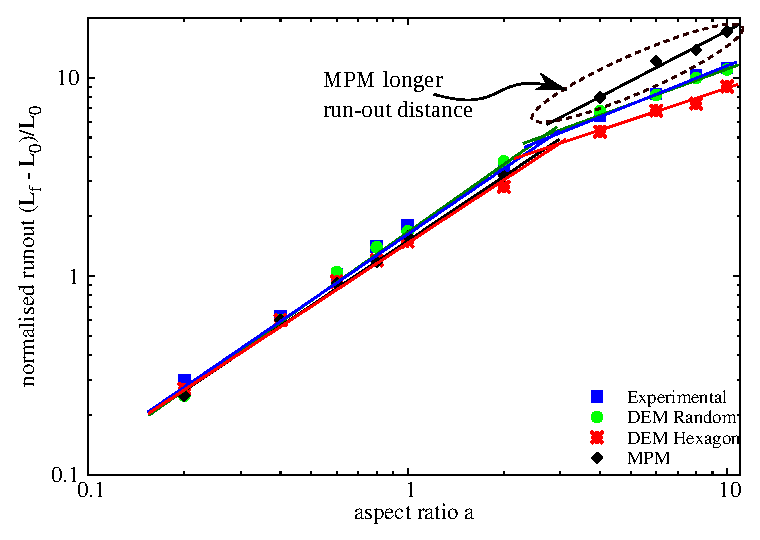
\includegraphics[width=\textwidth]{runout}
\caption{Normalised final runout distance for columns with different initial 
aspect ratio}
\label{fig:runout}
\end{figure}

\begin{figure}[tbhp]
\centering
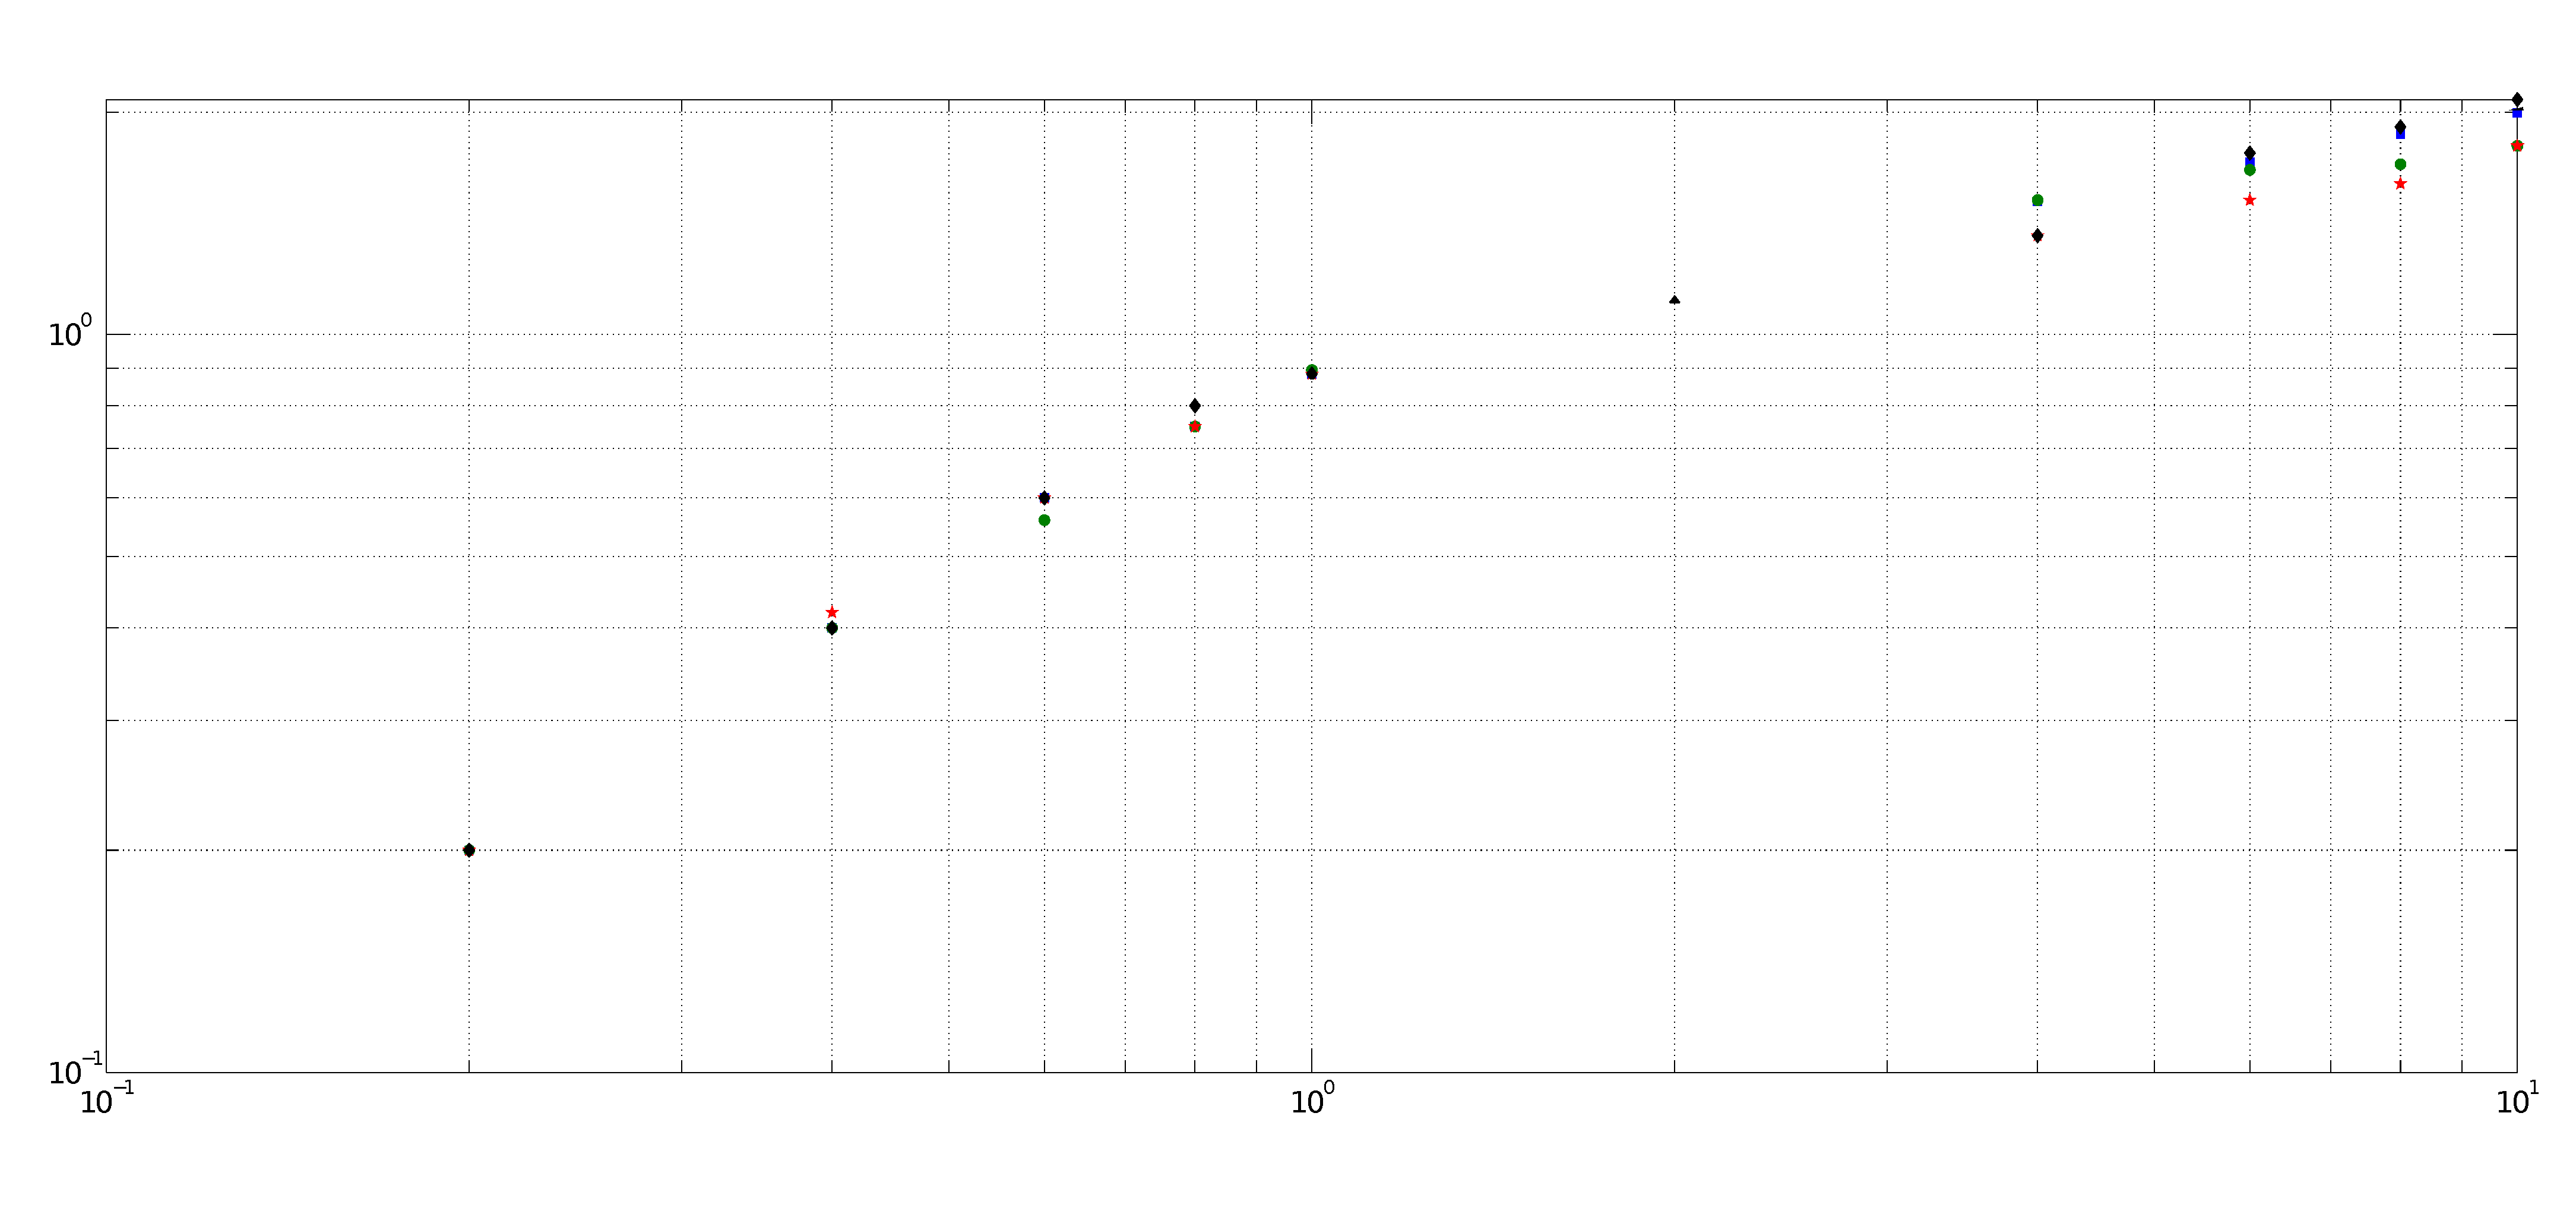
\includegraphics[width=\textwidth]{height}
\caption{Normalised final collapse height for columns with different initial 
aspect ratio}
\label{fig:height}
\end{figure}

\subsection{Flow evolution and internal flow structure}
For a fixed granular material and substrate properties, the flow dynamics and 
the final deposit morphology do not depend on the volume of granular material 
released, but depend only on the aspect ratio `\textit{a}' of the column. A 
power law relationship is observed between the run-out distance and the initial 
aspect ratio of the column. A transition in the run-out behaviour at an aspect 
ratio of 2.3 indicates a change in the flow dynamics. For smaller aspect 
ratios, the granular mass fails through avalanching of flanks producing a 
truncated cone-like deposit (`\textit{a}' < 0.7) or conical deposit 
(`\textit{a}' > 0.7). At smaller values of aspect ratios, the flow is initiated 
by failure at the edge of the pile along a well-defined fracture surface. The 
grains located above the failure surface move ``\textit{en masse}'' leaving a 
static region underneath the failure surface. After a transient time of order 
$\tau_{c}$, defined as $\sqrt{H_{\textit{i}}/g}$, the flow is fully developed. 
The velocity profile along the granular column at critical time $\tau_{c}$ is 
presented in Figure~\ref{fig:a04tc}. At critical time, the velocity field 
depends only on the position of the grain along the sliding mass. The maximum 
velocity is observed at the front of the flowing mass corresponding to that of 
a plug flow in horizontal direction. Particulate and continuum simulations 
yield similar run-out distance at critical time. Unlike particulate 
simulations, the Material point method predicts that the maximum horizontal 
velocity occurs at the top of the sliding mass. Behind the fast flowing front, 
the flow is localized in the mass above the failure surface and the velocity 
profiles are locally parallel to the failure plane. The flow is composed of 
upper linear part and a lower exponential tail in the static granular bed. The 
velocity profile is similar to steady granular surface flow as observed 
by~\citet{Lajeunesse2004}. 

For columns with lower initial aspect ratios, the run-out distance is 
proportional to the mass flowing above the failure surface. To understand the 
amount of mass mobilized during a collapse, the angle of the failure surface 
has to be studied. Figure~\ref{fig:a04tc} shows a distinct failure surface 
when the flow is fully developed at critical time $\tau_{\textit{c}}$. The 
angle of the failure surface is found to be about $55^{o}$. The failure surface 
begins from the toe of the column and protrudes inwards at an angle of 50 to 
$55^{o}$. For columns with lower aspect ratios, the formation of the 
``truncated conical deposit'' or ``conical deposit'' depends only on the 
initial length of the column, as the angle of the failure surface is found to 
be independent of the aspect ratio. The failure angle is consistent with the 
interpretation in terms of \textit{active Coulomb 
failure}~\citep{Lajeunesse2004}, which leads to a predicted failure angle 
$\theta_{\textit{y}}=45^{o}+\delta / 2$, where $\delta$ is the internal 
friction angle of the granular material. In the present study, the friction 
angle of the glass beads is $22^{o}$, which leads to 
$\theta_{\textit{y}}=45^{o}+22^{o}/ 2=56^{o}$, which is in good agreement with 
the numerical simulations and experimental observations 
by~\citet{Lajeunesse2004}. Contrary to the suggestion 
of~\citet{Lajeunesse2004}, the fracture angle is found to have no direct effect 
on the transition between the truncated cone and the conical deposit occurring 
at an aspect ratio of 0.7.~\citet{Schaeffer1990} observed the onset of 
instabilities in a narrow wedges of $56\mbox{ to }65^{o}$ for Cambridge type 
constitutive models that describes granular flows. This observation matches 
well with the failure angle observed in the present study. The final profile of 
the collapsed granular column with an initial aspect ratio of 0.4 is shown in 
Figure~\ref{fig:a04f}. The failure surface is distinct and the hexagonal dense 
packing of grains has a steeper failure surface in comparison with the random 
packing. The variation observed in the angle of the failure surface causes a 
difference in the amount of mobilized mass above the failure surface, and in 
turn in the run-out distance. The lower value of run-out distance observed in 
the case of hexagonal packing of grains can be attributed to the 
crystallisation effects. crystallisation is the formation of large-scale 
lattice structures during the flow, resulting in non-generic flow patterns. 
crystallisation is found to have a significant effect on the final state of the 
granular column.~\citet{Lacaze2009} observed that poly-disperse grains have 
lesser tendency to crystallize especially in the case of columns with larger 
aspect ratio. 

\begin{figure}[tbhp]
\centering
\includegraphics[width=\textwidth]{a04tc}
\caption{Velocity profile of a granular column collapse ($`a' = 0.4 \& 
t=\tau_c$)}
\label{fig:a04tc}
\end{figure}



\begin{figure}[tbhp]
\centering
\includegraphics[width=\textwidth]{a04f}
\caption{Velocity profile of a granular column collapse ($`a' = 0.4 \& 
t=3\times\tau_c$)}
\label{fig:a04f}
\end{figure}


For larger aspect ratios, the flow is still initiated by a well defined failure 
surface as can be seen in Figure~\ref{fig:a6tc}. However, in this case the 
initial granular column is much higher than the top of the failure surface. Due 
to gravity most of the grains in the column fall in the vertical direction 
consuming the column along their way. When they reach the vicinity of the 
failure surface, the flow gets deviated along the horizontal direction 
releasing a huge amount of kinetic energy gained during the free fall. For 
larger aspect ratio (\textit{a} > 0.7), the resulting static region is a cone, 
the final height of the cone, i.e, $\textit{H}_{\textit{f}}$ lies above the 
summit of the failure surface. Hence, a different evolution is observed from 
that of the axis-symmetric geometry~\citep{Lube2005}, where the final height 
coincides with the summit of the failure surface forming a truncated conical 
deposit.~\citet{Lajeunesse2004} articulated the variation in the deposit 
morphology between the axis-symmetric case and the rectangular collapse to be a 
geometrical effect rather than as an experimental artefact. The final profile 
of the collapsed granular column with an initial aspect ratio of 6 is presented 
in Figure.\ref{fig:a6f}. An initial failure surface starting from the toe end 
of the column at an angle of about 55$^{o}$ can be observed at critical time 
$\tau_{c}$. As the collapse of the granular collapse progresses, successive 
failure planes parallel to the initial failure surface are formed and shear 
failure occurs along these planes. The presence of several shear bands in the 
final profile of the collapsed granular column confirms the hypothesis. 
crystallisation in hexagonal packing causes a significant effect on the run-out 
distance by forming series of parallel shear bands. However, the Material Point 
Method fails to capture the formation of shear bands during the collapse. This 
observation throws light on the mechanics of propagation of shear bands in 
massive landslides such as the Storegga submarine landslide. The flow behaviour 
becomes similar to that of columns with lower aspect ratio as the flow starts 
descending along the failure plane. Regardless of the experimental 
configuration and the initial aspect ratio of the columns, the flow is 
initiated by a well-defined rupture surface, above which the material slides 
down leaving a static region underneath the failure plane. Depending on the 
aspect ratio of the column, two asymptotic behaviours are observed. For smaller 
aspect ratios, the flow is dominated by friction and by the pressure gradient 
for larger aspect ratio.

To study the flow dynamics of granular columns with different aspect ratios, 
the flow front \textit{L}(\textit{t}) and the maximum height of column 
\textit{H}(\textit{t}) are tracked. The evolution of scaled height 
$(H_{\textit{f}}/L_{\textit{i}})$ and the run-out distance 
$(L_{\textit{f}}-L_{\textit{i}})/L_{\textit{i}}$ with time for granular columns 
with an initial aspect ratio of 0.4 and 6 are presented in 
Figures.~\ref{fig:flowa04} and~\ref{fig:flowa6}. Time is scaled with respect to 
the critical time $\tau_{c}$, defined as the time at which the flow is fully 
mobilized. Three distinct regions can be observed in the flow evolution of 
granular column collapse regardless of the initial aspect ratio of the column. 
An initial transient acceleration phase is observed for a time 0.8$\tau_{c}$. 
This phase is followed by a heap movement of granular materials at the foot 
with a constant spreading velocity \textit{V} for about 2$\tau_{c}$. When time 
`\textit{t}' $> \tau_{c}$, the velocity varies linearly with depth in the 
flowing layer and decreases exponentially with depth near the static layer. 
This velocity profile is similar to those observed in steady granular surface 
flows~\citep{Lajeunesse2004}. Most of the run-out happens during this phase. 
The final phase involves deceleration of the flow front and the flow comes to 
rest after 0.6$\tau_{c}$. The spreading of the granular column ceases after a 
time in the order of 3$\tau_{c}$ for all values of aspect ratios, however some 
motion still persists along the free surface behind the flow front for a much 
longer time due to internal rearrangement, the duration of which can last up to 
$\textit{t} \approx 6\tau_{c}$. For smaller aspect ratios, the critical time is 
evaluated as the point of intersection of the scaled run-out and height. The 
critical time predicted for both hexagonal and random packing of grains matches 
the experimental observations. However, the Material Point Method overestimates 
the critical time by a factor of 1.25, which means that it takes longer for the 
flow to be fully mobilized. However, the actual run-out duration is short and 
the granular materials comes to rest abruptly at about $\textit{t}=3\tau_{c}$. 
For columns with larger aspect ratios, the continuum and particulate approaches 
simulate similar flow evolution behaviour for times up to 3$\tau_{c}$, beyond 
which particulate simulations stabilise and come to rest, while the flow 
continues to evolve in MPM simulations resulting in larger run-outs than 
expected. The flow tends to come to rest at time $\textit{t}=6\tau_{c}$. The 
three phases in a granular flow can be distinctly observed in the flow 
evolution plot for a granular column with initial aspect ratio of 6 (see 
Figure~\cref{fig:flowa6}). For larger aspect ratios, the flow evolution 
behaviour 
observed in the case of random packing matches the experimental observation 
by~\citet{Lajeunesse2004}. Hexagonal packing predicts longer time for the flow 
to evolve, which can be attributed to the increase in the internal resistance 
due to crystallisation of grains. MPM overestimates the critical time by 50\%, 
however has the same value of run-out as the particulate simulations, at time 
$\textit{t}=3\tau_{c}$, beyond which the material continues to flow until it 
ceases at 6$\tau_{c}$. In order to understand the flow dynamics in the case of 
Material Point Method it is important to study the effect of different 
parameters on the deposit morphology. 

\begin{figure}[tbhp]
\centering
\includegraphics[width=\textwidth]{a6tc}
\caption{Velocity profile of a granular column collapse ($`a' = 6 \& 
t=\tau_c$)}
\label{fig:a6tc}
\end{figure}

\begin{figure}[tbhp]
\centering
\includegraphics[width=\textwidth]{a6f}
\caption{Velocity profile of a granular column collapse ($`a' = 6 \& 
t=3\times\tau_c$)}
\label{fig:a6f}
\end{figure}

%\begin{landscape}
%\centering

%\end{landscape}

\begin{figure}[tbhp]
\centering
\includegraphics[width=\textwidth]{flowa04}
\caption{Flow evolution of a column with $`a'=0.4$}
\label{fig:flowa04}
\end{figure}

\begin{figure}[tbhp]
\centering
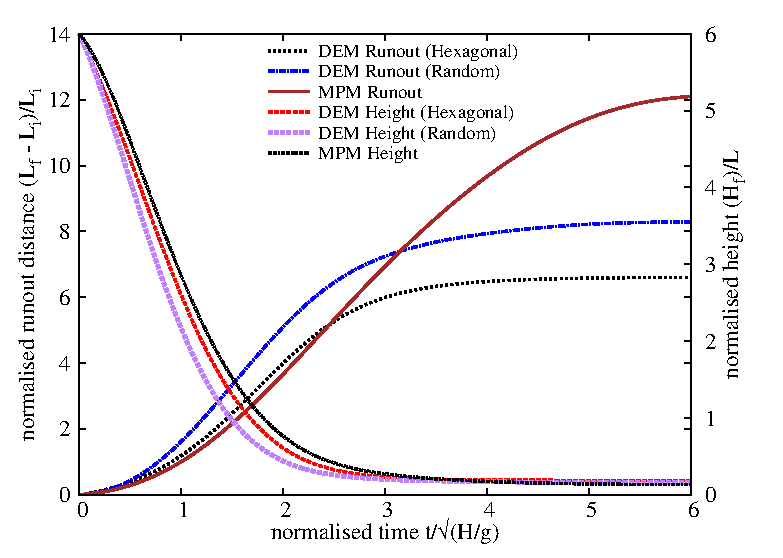
\includegraphics[width=\textwidth]{flowa6}
\caption{Flow evolution of a column with $`a'=6$}
\label{fig:flowa6}
\end{figure}

\subsection{Energy dissipation mechanism}
\label{sec:energy}
The time evolution of the flow exhibited three distinct stages during the 
collapse of a granular column. Studying the energy dissipation mechanism 
provides useful insight into the flow dynamics. %TODO: Add figure
shows 
the time evolution of potential energy $(E_{p})$ and kinetic energy $(E_{k})$ 
normalized by the initial potential energy $E_{o}$.
\begin{align}
& 
\textit{E}_{\textit{p}}=\sum\limits_{\textit{p}=1}^{\textit{N}_{p}}{\textit{m}_{p}\textit{g}\textit{h}_{p}}
 \\
& 
\textit{E}_{\textit{ki}}=\frac{1}{2}\sum\limits_{\textit{p}=1}^{\textit{N}_{p}}{\textit{m}_{p}\textit{v}_{\textit{p}}^{2}}
\end{align}
where $\textit{N}_{p}$ is the total number of particles, $\textit{m}_{p}$ is 
the mass of a particle `\textit{p}', $\textit{h}_{p}$ is the height and 
$\textit{v}_{p}$ is the velocity of the particle `\textit{p}'. It can be 
observed from the figure that the initial potential energy stored in the 
particle is converted to kinetic energy which is dissipated as the granular 
material flows down. Three successive stages can be identified in the granular 
column collapse. In the initial acceleration stage $(\textit{t}<0.8\tau_{c})$, 
the initial potential energy stored in the grains is converted into vertical 
motion. In the second stage, the grains undergo collisions with the bottom 
plane and/or with neighbouring grains, and the stored potential energy is 
converted into horizontal motion. In the third stage, the grains eventually 
leave the base area of the column and flow sideways. As the process involves 
collective dynamics of all the particles, it is difficult to predict the exact 
trajectory of a grain, however, the overall dynamics can be explained. To 
explain the dissipation of energy during the collapse,~\citet{Staron2005} 
assumed that the total initial potential energy stored in the system is 
completely dissipated through friction over the entire run-out distance as:
\begin{align}
\mu \textit{m}_{o}g \times (L_{f}-L_{i}) = \textit{m}_{o}g \textit{H}_{o}
\end{align}
where $\mu$ is the friction coefficient. The model predicts well the flow 
dynamics for columns with larger aspect ratios, as most of the initial 
potential energy is dissipated during the collapse involving the entire column. 
However, for columns with smaller aspect ratios, only a portion of the mass 
above the failure surface is involved in the flow. Hence, the energy 
dissipation should involve only the grains lying above the failure surface. A 
mathematical model, which considers the grains lying above the failure surface, 
will be derived to predict the flow dynamics of the granular column collapse 
for different aspect ratios. 